\shorthandoff{:!} %règle un problème de compatibilité avec babel
%
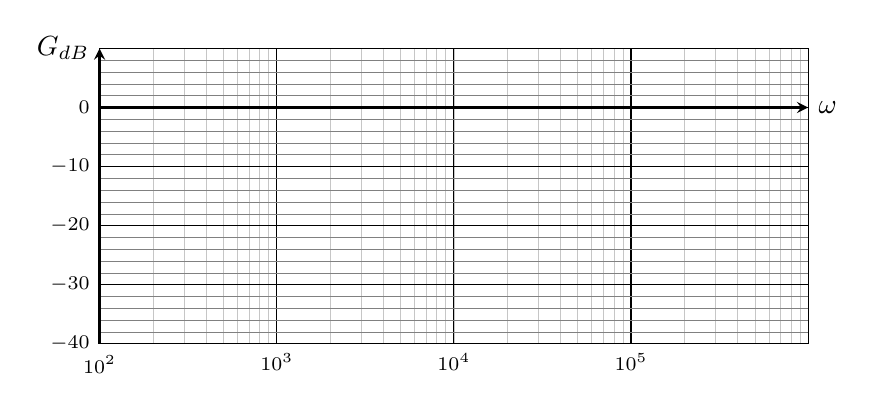
\begin{tikzpicture}[scale=0.75,rotate=0]
	% Dimensions du repere
	\def\xlrg{12} \def\ylrg{5}
	%
	% Tracé de l'axe log base 10
	\foreach \ee in{0,1,2,3}{
		\foreach \x in {1,2,...,10} {
			\draw[very thin,color=gray!45] ({\xlrg/4*ln(\x*10^\ee)/ln(10)-\xlrg},0)--({\xlrg/4*ln(\x*10^\ee)/ln(10)-\xlrg},-\ylrg);
		};
	};
	%tracé de la légende pour les puissances de 10
	\foreach \ee in{3,4,5}{
		\foreach \x in {10}
		{\draw[thin,color=black]({\xlrg/4*ln(\x^(\ee-2))/ln(10)-\xlrg},0)--({\xlrg/4*ln(\x^(\ee-2))/ln(10)-\xlrg},-\ylrg) node [below] {\scriptsize $10^{\ee}$};
		};
	};
	\node at (-\xlrg,-\ylrg-0.35) {\scriptsize $10^2$};
	% Grille lineaire
	\draw [xstep=\xlrg,ystep=.2,gray,very thin] (-\xlrg,-\ylrg) grid (0,0); 
	\foreach \ee in{-40,-30,...,0}{\draw [color=black](0,{-\ylrg+(\ee+40)/10})(-\xlrg,{-\ylrg+(\ee+40)/10}) node [left] {\scriptsize $\ee$};
	};
	\draw [xstep=\xlrg,ystep=1,color=black] (-\xlrg,-\ylrg) grid (0,0);
	%
	% Légende des axes
	\draw[thick,->,>=stealth](-\xlrg,-\ylrg+4) -- (0,-\ylrg+4) node[right] {$\omega$};
	\draw[thick,->,>=stealth] (-\xlrg,-\ylrg) -- (-\xlrg,0) node[left] {$G_{dB}$};
\end{tikzpicture}
\shorthandon{:!}

